\section{Introduction}

Data, curated by journalists, scientists and policy makers into charts and other visual summaries, is how we understand the changing world around us. But charts can be hard to interpret correctly, even with access to the relevant data source. Innocent (but devastating) mistakes such as transposing two columns of data may go unnoticed for several years, even in widely cited papers~\cite{miller06}. Less innocent mistakes are deployed by politicians to mislead voters \cite{fullfact19}. Understanding and trusting a visualisation, even for an expert, means knowing what its visual attributes actually \emph{represent}, which in turn involves the following two comprehension challenges:

\begin{enumerate}
  \item Identifying the mapping between data source and visual elements in the visualisation
  \item Understanding how different views of the same data are related
\end{enumerate}

\noindent Even with the data and source code used to create the visualisation to hand, answering questions such as these is difficult, requiring time and expertise. The basic problem is that visualisations are opaque, disconnected from the data and computations used to create them. This situation would be significantly imporved if visualisations allowed a reader to explore the relationship to the underlying data through the visualisation itself, revealing the relevant connections on a need-to-know basis, as the reader interacts with it (\figref{introduction:data-linking} below):

\begin{figure}[H]
   {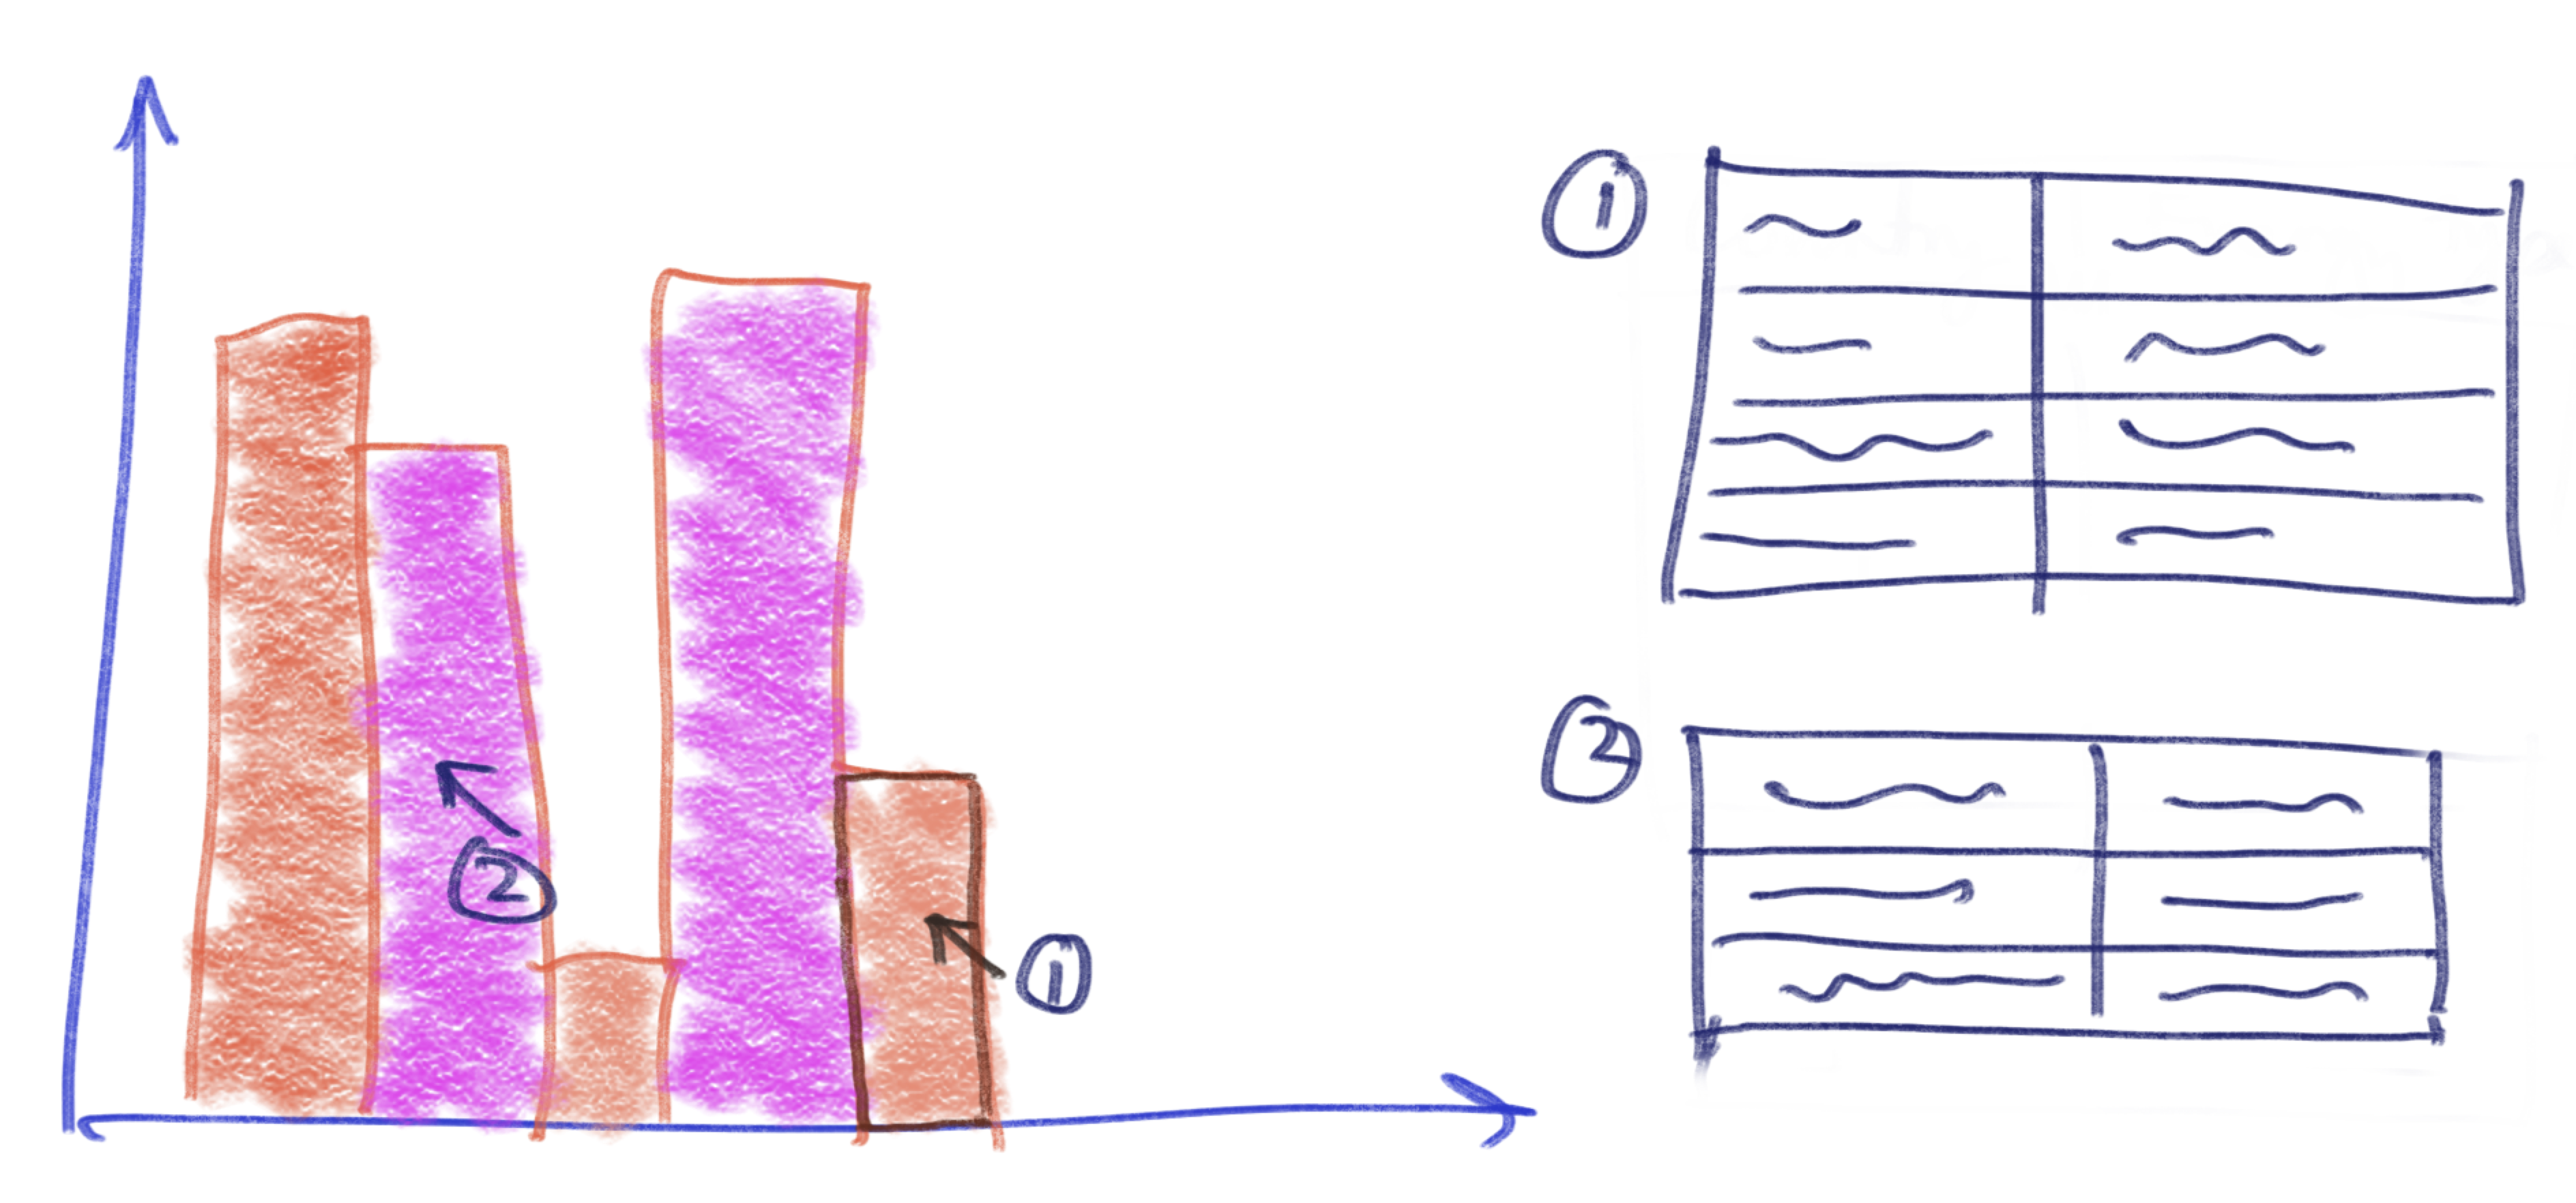
\includegraphics[scale=0.07]{fig/example/data-linking.png}}
   \caption{Data visualisation with fine-grained data linking}
   \label{fig:introduction:data-linking}
\end{figure}

Building this sort of ``data-linked'' visualisation by hand is possible, but is a significant undertaking, requiring intimate knowledge of the computational relationship between chart and data, and programming effort to expose that information to the reader. Manual approaches are also unlikely to be correct and lead to brittle solutions that need to be changed whenever the application logic changes. Given that a visualisation is a view computed from a data source, it seems plausible that we might adapt techniques from program analysis and data provenance to provide a runtime infrastructure that automatically supports linked selections. Then the data scientist or visualisation designer can concern themselves with cleaning, aggregating and presenting data, leaving the infrastructure to take care of linking visualisations to the underlying data sources.

\subsection{Linking visualisations to each other}

It is also common to use more than one view to present distinct but related aspects of data. (We say visualisations are \emph{cognate} when they are related in this way.) Geospatial applications like GeoDa \cite{anselin06} and charting libraries like Plotly provide a view coordination feature called \emph{brushing and linking} \cite{becker87}, where selections in one chart automatically select corresponding elements in the other, as an aid to comprehension. In \figref{introduction:vis-linking} below, selecting a bar on the left automatically selects all the related visual elements on the right. Although such coordination features are highly desirable, they are either baked into specific applications, or require programmer effort and therefore must be anticipated in advance by the chart designer. Moreover the linking is opaque, providing no direct way for the reader to see the data which underpins the relationship.

\begin{figure}[H]
   {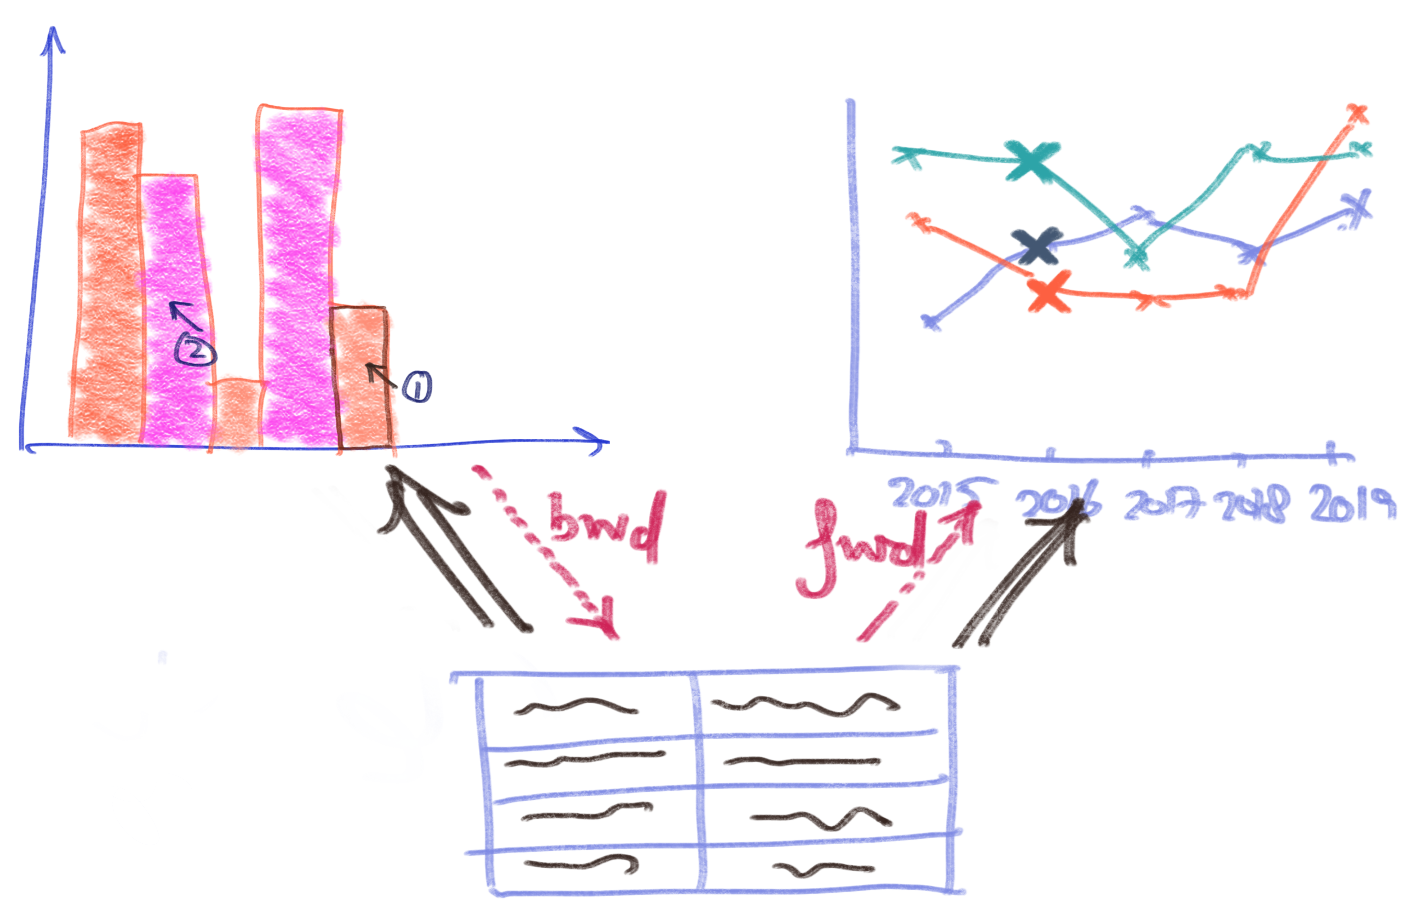
\includegraphics[scale=0.14]{fig/example/vis-linking.png}}
   \caption{Linking cognate visualisations via common data dependencies}
   \label{fig:introduction:vis-linking}
\end{figure}

\subsection{Our contributions}

In this paper, we present new language-based data provenance techniques for linking visualisations to data, and to each other, in a fine-grained way. Our specific contributions are as follows:

\begin{itemize}[leftmargin=*]
   \item[--] a review of \emph{Galois slicing}, a program slicing framework with round-tripping properties appropriate to our problem, and an analysis of its shortcomings (\secref{background});
   \item[--] a new bidirectional dependency analysis inspired by Galois slicing, addressing these shortcomings, for a core calculus with lists and arrays (\secref{core-language});
   \item[--] a surface language called \OurLanguage with familiar functional programming features, including piecewise definitions, pattern matching, list notation and list comprehensions, and an extension of our analysis to the desugaring (\secref{surface-language});
   \item[--] an implementation of Fluid in PureScript, and a discussion and evaluation of the strengths and weaknesses of our approach (\secref{implementation}).
\end{itemize}
